\documentclass[11pt]{book}
\usepackage{array}           % For double-column exercises.
\usepackage{longtable}       % For double-column exercises.
\usepackage[normalem]{ulem}  % For strikethrough.
\usepackage{paralist}       
\usepackage{enumitem}        % To "resume" enumerated lists.
\usepackage{epsfig}       
\usepackage{afterpage}       
\usepackage{multicol}       
\usepackage{fancybox}       
\usepackage{makeidx}       
\usepackage{textcomp}
\usepackage{fancyvrb}
\usepackage{footnote}
\newcommand{\freakingtilde}{\raisebox{0.5ex}{\texttildelow}}
\makesavenoteenv{tabular}  % to allow footnotes in tables

%\usepackage{enumerate}       

\makeindex 

\newenvironment{custommargins}[2]%
  {\addtolength{\leftskip}{#1}\addtolength{\rightskip}{#2}}{\par}

% Set left margin - The default is 1 inch, so the following
% command sets a 2-inch left margin.
\setlength{\oddsidemargin}{1in}
\setlength{\evensidemargin}{0in}
% Set width of the text - What is left will be the right margin.
% In this case, right margin is 8.5in - 1.25in - 6in = 1.25in.
\setlength{\textwidth}{5.5in}

% Set top margin - The default is 1 inch, so the following
% command sets a 0.75-inch top margin.
\setlength{\topmargin}{.75in}

% Set height of the text - What is left will be the bottom margin.
% In this case, bottom margin is 11in - 0.75in - 9.5in = 0.75in
\setlength{\textheight}{7.25in}
\usepackage{amsmath,amsthm,amsfonts,amssymb,latexsym}

\setlength{\parindent}{0pt}
\setlength{\baselineskip}{1.5pt}
\setlength{\parskip}{6pt}

\begin{document}

\title{Blueprints: Creating, Describing, and Implementing\\Designs for Larger-scale Software
Projects\\{\small version 1.0.0}}
\author{Stephen Davies, Ph.D.\\Computer Science Department\\University of Mary Washington}
\date{}
\maketitle

\frontmatter

\renewcommand{\contentsname}{Contents at a glance}

\setcounter{tocdepth}{0}
\tableofcontents

% 
\chapter{Preface}
Coming soon.


\setcounter{chapter}{1}

\mainmatter
%
\chapter{Getting off the ground}
\label{ch:gettingOff}

\index{command line}
\index{Linux}
\index{Unix}
Before we begin our study of object-oriented systems proper, we'll introduce
the command-line toolset we'll be using to construct our programs. We'll take
each of the most important tools out of our toolbox, lay them out before us on
a little mat, and learn what they're for.

\section{Why the command line?}

\index{CLI (command-line interface)}
\index{GUI (graphical user interface)}
Developing software in a command-line environment (sometimes abbreviated
``CLI'' for \textbf{command-line interface}, as opposed to a
``GUI\footnote{Commonly pronounced ``gooey.''}'' or \textbf{graphical user
interface}) involves typing white text in little black boxes. It requires
memorizing and regurgitating a variety of obscure commands. It demands exact
adherence to an inconsistent syntax, and exacts heavy penalties for mistakes,
all while providing only a very crude and clunky-looking interface.

It's natural to wonder why we would want to do this. After all, aren't
computer systems immeasurably more sophisticated now? If even end users run
fancy, graphical, forgiving apps, shouldn't computer scientists expect even
easier-to-use and sexier-looking stuff?

It may seem so, and in terms of the \textit{power} the tools provide, we'll
discover that indeed software developers are aptly equipped. But in some ways
it's a false expectation to assume that our toolset would be as \textit{easy}
to operate as that of an everyday user. After all, which is easier: to drive a
car, or to be a mechanic? Even though I enjoy cruise control and
auto-adjusting seats, I don't find it strange at all to learn that mechanics
still use socket wrenches to adjust piston assemblies.

Much of what makes a CLI so powerful is its expressiveness. A driver can press
any of the three or four cruise control functions the manufacturer provided.
But a mechanic can take any of hundreds of tools, tweak dozens of different
parts, and combine these adjustments in uncountable ways. That's the kind of 
flexibility the command line provides.

The difference between a CLI and a GUI is that with the latter, the user can
essentially do \textit{only what the tool designer anticipated she would want
to do.} There's no way she can express something that isn't one of the
tailor-made menu options.

When you use the command line, think of it as composing sentences, word by
word. A GUI comes with a repertoire of standard sentences you can choose from.
That makes it easy to do standard things, and hard to make silly mistakes. But
a CLI, being inherently language-based, is immeasurably more flexible. You can
write any (legal, grammatically correct) sentence you choose, even one the
designers of the CLI never thought of, and even one that you didn't know you'd
want to type until a moment ago. The bits and pieces can be combined in a
myriad of ways, just as nouns and verbs can.

\index{Finlayson, Ian}
There are other reasons as well that many developers live on the command line.
Among them are\footnote{Thanks to Ian Finlayson for capturing much of this
list.}:

\begin{itemize}
\itemsep.1em

\item \textbf{Speed.} It turns out to be way, way faster to type commands --
in combination with the various shortcuts and recall/edit operations -- than
it is to sift through menu options and such with a mouse. Trust me.

\index{remote access}
\index{shell}
\item \textbf{Remote access.} When you're running programs on your own device,
it's possible to do it with a GUI. But computer scientists very often have to
connect over the network to distant machines in order to tell them what to do.
Every time you need to configure a web server, for instance, or update a
publicly-accessible database, or run a time-consuming job on a parallel
cluster, or correct the data on your mobile device, you need a way to issue
commands to another machine through a very low-bandwidth channel. Opening a
command line ``shell'' to that remote device is by far the most common and
effective way to do this.

\index{scriptability}
\item \textbf{Scriptability.} There's just no good way to automate a sequence
of GUI operations. To explain to someone else how to accomplish something, you
have to painfully walk them through each operation (``go to the Start menu and
find Accessories, then in the Math menu choose Calculator...when it comes up,
right-click in the background and enable Advanced Options...'') which is
tedious and error-prone. It'd be nice if you could just send them a custom
command which would do all that. As a matter of fact, it would be nice if
\textit{you} could make a custom command which would do all that, so that you
could execute it many times without rehashing the same rigmarole. You'll find
that CLIs are eminently automatable in this way. You can create custom
commands called ``scripts'' that are combinations of other interacting
commands, and in this way you become master of your whole world.

\index{Cygwin}
\index{Mac OS X}
\index{Microsoft Windows}
\index{Raspberry Pi}
\index{Kindle}
\index{Terminal application}
\item \textbf{Consistency.} Graphical user interfaces are more different from
each other than CLIs are. Partly this is because nearly any CLI you're likely
to use is Unix/Linux-based\footnote{For our purposes, you can consider the
terms ``Unix'' and ``Linux'' exact synonyms. The Mac OS X command line
(available through the ``Terminal'' app) is Unix-based, too. Windows machines
aren't, but programs like ``Cygwin'' can be downloaded for free and provide a
Linux-like command-line veneer over the operating system.}, and hence they all
``speak the same language.'' It's great to be able to log on to different
laptops, web servers, your phone, your Kindle, or a Raspberry Pi and get the
same prompt that understands the same stuff.

\index{Linux}
\index{Unix}
\index{CLI (command-line interface)}
\item \textbf{Stability.} CLIs rarely change. When they do, it's very very
rarely in a non-backwards-compatible way. Every time a new graphical user
interface is released, you have to go through a period of hunting around and
finding out where everything is. With Unix/Linux, you can literally run
commands that were written last century and they will likely still work as is.

\end{itemize}

There's always a few students who despite the above benefits, resist learning
this material at first. I get it. It's like learning a new language, and the
immense effort to understand an alien world sure doesn't feel like it's going
to pay off any time soon. All I can say is that if you're not convinced it's
worth it, for now just think of it as something you have to master ``just
because your professor and the industry says so.'' My hope is that by the end
of this course, you're pleasantly surprised by seeing some payoff for your
hard work.


\section{The filesystem}
\index{filesystem}
\index{file}
\index{tree}
\index{directory}
\index{folder}

Okay. The backdrop for all our use of the Linux command-line interface is the
\textbf{filesystem}.\footnote{Often, not always, written as a single word as I
have it here.} Any general-purpose computer, no matter its architecture or OS,
has an area of permanent storage for user data. Interestingly, and
conveniently, they're all organized in pretty much the same way: as a
\textbf{tree} of \textbf{files} and \textbf{directories}. (Windows/Mac users
will be familiar with the term ``\textbf{folder},'' which \textit{means exactly
the same thing as ``directory.''}) In what follows, we'll be using a different
syntax (text instead of visual icons) to work with what is conceptually the
same organizational structure you're used to on your own computer.

\subsection{Files and directories}

\index{filesystem extension}
A file is simply any named chunk of stuff on your disk. Images, .mp3 tunes,
Word docs, and (importantly) plain text files are all in this category. On
Windows, you're used to each of these files having a filesystem ``extension''
designating its type: ``.doc'' means a Word doc, and ``.jpg'' means an image
file, for example. This is sort of true with Linux, although the rules are
a bit looser. Not all files have extensions at all, and when they do, it's
more a signal that they're intended to be treated a certain way than a
hard-and-fast requirement.

\index{java file@\texttt{.java} file}
The most important files you'll work with in this class will have a
\texttt{.java} extension. These are your Java source files. You'll also work
with other various supporting files to make all the tools work correctly.
It's important to realize that \textit{a file is fundamentally just some data,
which can theoretically be opened and dealt with by any program}. When we say
that HamletPaper.doc ``\textit{is}'' a Word doc, what we really mean is that
its data is formatted in a certain way that the Microsoft Word application
expects to see, so it can render it on the screen for editing. But it is
possible to open that same HamletPaper.doc file with other programs and
manipulate its contents. This may seem sketchy, but it is actually a force for
good.

In particular, you'll be tempted this semester to think of a \texttt{.java}
file as ``a \texttt{vim} file,'' in the same way that you may think of an
\texttt{.xls} file as ``an Excel file.'' I hope to eventually break you of this
habit, as you learn to see files as text or data that is actually independent
of what kind of program might be used to open and manipulate it.

\index{directory}
A directory is a container for files \textit{and also other directories}. That
last italicized phrase is what gives rise to the overall tree structure of the
filesystem, as discussed in the following section.

\index{Foreman, George}
By the way, every file and directory \textit{in a particular directory} must
have a unique name. You can't have a file called ``DireStraits.mp3'' and
another one also called ``DireStraits.mp3'' sitting there in the same folder:
it's a name collision. However, it's perfectly permissible to have two files
with the same name in different directories. This is kind of like how there
isn't more than one ``Stephen'' in my immediate family (that would be
confusing\footnote{With apologies to boxing legend George Foreman, who named
all four of his children ``George.'' That practice is not
filesystem-compatible.}), but there are of course many ``Stephens'' in the
world.

\subsection{The filesystem tree}

\index{tree}
\index{filesystem}
\index{directory!parent}
\index{parent directory}
The files and directories in a filesystem form a nested, hierarchical
structure called a \textbf{tree} (see Fig.~\ref{fig:tree}). I have drawn two
kinds of nodes in this tree: directories (yellow ovals) and files (blue
boxes). As expected, some of the directories have arrows coming out of them,
but none of the files do. The elements that a directory is pointing to are the
contents it contains: \textit{e.g.}, the left-most ``\texttt{america}''
directory contains another directory (``\texttt{nation}'') and also the file
\texttt{A.txt}. We use the term \textbf{parent directory} to mean the
directory immediately above an entry in the filesystem; the left-most
\texttt{A.txt} file's parent directory is the \texttt{america} directory we
just spoke of.

\begin{figure}[ht]
\centering
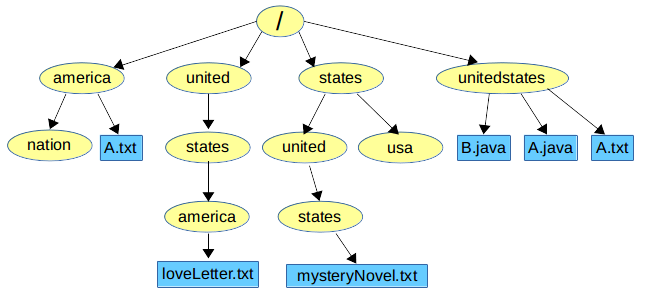
\includegraphics[width=0.9\textwidth]{tree.png}  %650x300
\caption{The Linux filesystem, in pictorial form.}
\label{fig:tree}
\end{figure}

Note that in order to keep you on your toes, I've given several entries in
this example filesystem the same name: in addition to a couple different
\texttt{america}s, we've got several \texttt{states}, multiple different
\texttt{A.txt}s, etc. In no case, however, are the duplicately-named entries
in the same directory. (Convince yourself of that fact.)

\subsubsection{Only one surprise}

\index{Microsoft Windows}
So far this is pretty easy. And it won't get much harder. But here's the one
thing you have to get used to: with a CLI, \textit{we won't ever actually see
that filesystem picture visually.} It's there, but we don't explicitly view it
in graphical form. Instead, there will be a textual way of referring to every
file and directory. It's straightforward, but can be a bit of a shock to those
coming from point-and-click systems like Windows.

\subsection{The ``current'' (or ``working'') directory}

\index{directory!current}
\index{directory!working}
\index{current directory}
\index{working directory}
One vital concept to grasp is that every time we issue a command or run a
program in Linux, we are doing so \textit{within the context of a particular
directory}. Conceptually, we think of being ``in'' a certain directory at any
point in time. We call this directory ``the \textbf{current directory}'' or
``the \textbf{working directory}'', and we'll learn commands to find out what
it is and to change it to something else.

Which one we're ``in'' has a crucial impact on what happens when we execute a
command. For instance, if our current directory is the far-left
\texttt{america} directory, and we issue a command that does something to
``\texttt{A.txt}'', it would act on the left-most \texttt{A.txt} file, since
it's the one within the current directory. But if our current directory were
\texttt{unitedstates}, ``\texttt{A.txt}'' would instead mean the far-right blue
node.

I've found that failure to understand the current directory is one of the most
common trouble spots for beginning Linux programmers.

\subsubsection{The root directory}

\index{directory!root}
\index{root directory}
\index{tree}
Okay, back to the filesystem as a whole. At the top of the tree is the
\textbf{root directory}, which has no parents. (This is often disorienting to
non-computer-scientists, since in the real world trees actually grow
\textit{up}, not down. But in computer science, we always draw trees growing
down from the root.)

\index{backslash}
\index{forward slash}
\index{slash}
\index{Microsoft Windows}
The root directory is the anchor point of the entire filesystem: it ultimately
contains everything under it. It also has a very strange name: ``\texttt{/}'',
pronounced ``slash.'' (This is a ``forward slash,'' by the way, to the left of
your right-most Shift key, not a ``backslash.'' Oddly, most Windows systems
use a backslash ``\texttt{\textbackslash}'' for this instead.) Stay awake,
because this ``\texttt{/}'' character will shortly mean something very
different as well.

\subsubsection{Paths}

\index{path}
\index{directory}
\index{file}
It should be apparent to you that as a consequence of this nested tree
structure, you can ``reach'' every element from the root directory by
traversing from arrow to arrow. Furthermore, you can do so in only one way.
For instance, the \texttt{B.java} file can be reached from the root by going
from ``\texttt{/}'' to \texttt{unitedstates} to \texttt{B.java}. And that's the
\textit{only} way to get there. You can reach \texttt{loveLetter.txt} by going
from ``\texttt{/}'' through \texttt{united}, \texttt{states}, and
\texttt{america}, in that order. This is true for every file and directory.

What this means is that every entry has a unique \textbf{path}, and we can
express it in text as well as in a diagram. Take the \texttt{B.java} file for
example. Its path is:

\quad\quad \texttt{/unitedstates/B.java}

\index{slash}
Look very carefully at that string as we dissect it. The most important thing
to grasp is that the two slash (``\texttt{/}'') characters \textit{each mean
something different}. The first one means ``the root directory, which is
called slash.'' But the second one is merely a separator, delimiting the
\texttt{unitedstates} from the \texttt{B.java}. So this path means
``\textit{start at the root directory}, go down to its \texttt{unitedstates}
entry (which is a directory), and there you have the \texttt{B.java} file.''

Similarly, the path to \texttt{loveLetter.txt} is:

\quad\quad \texttt{/united/states/america/loveLetter.txt}

\index{slash}
(Note that the slash between \texttt{united} and \texttt{states} makes all the
difference in the world: if it weren't there, we'd be starting our descent
through the right-most \texttt{unitedstates} directory as before.)

\index{path!absolute}
\index{absolute path}
\index{planet}
\index{path!relative}
\index{relative path}
These paths are called \textbf{absolute paths} because they \textit{start with
a slash}. This means that they give the complete, start-from-the-top position
of a particular file or directory. It's kind of like referring to a building
by its complete address, including city, state, zip code, country, and planet.
Often we want a short-hand way of referring to an entry without specifying its
entire absolute path. To do so, we use a \textbf{relative path}.

\index{directory!current}
\index{current directory}
A relative path is relative \textit{to the current directory}. And it does
\textit{\textbf{not}} begin with a slash. Instead, it gives directory names,
separated by slashes, indicating where to start descending \textit{from the
current directory}.

For example, let's say the current directory was ``\texttt{/states}''. And
suppose I used this relative path:

\quad\quad \texttt{united/states/mysteryNovel.txt}

(Note \textit{carefully} that it has \textit{no} initial slash!) This relative
path would instruct us to \textit{start at the current directory}
(\texttt{/states}) and from there traverse down to \texttt{united},
\texttt{states}, and then finally \texttt{mysteryNovel.txt}. Obviously, where
you end up is critically dependent on where you start -- on what the current
directory is.

\index{directory!current}
\index{current directory}
To test your understanding, realize that in this case where the current
directory is \texttt{/states}, there is no such file called
\texttt{united/states/america/loveLetter.txt}. In fact, even 
\texttt{united/states/america} doesn't exist. However, if we changed the
current directory to be the root (``\texttt{/}''), suddenly the relative path
\texttt{united/states/ america/loveLetter.txt} would be legit.

\section{Linux A-B-C's}

\index{Unix}
\index{Linux}
\index{filesystem}
\index{file}
\index{directory}
With the filesystem always hovering in the background, let's introduce the
first basic Linux commands to work with the files and directories. These
commands are so basic that they're like the alphabet of speaking any Linux
sentence. Using them should eventually be as familiar and effortless as
clicking the mouse.

\index{prompt}
\index{dollar sign (\texttt{\$})}
In all that follows, I will precede anything you are to type on the Linux
command line with a dollar sign \textbf{prompt}:

\begin{Verbatim}[fontsize=\small]
$
\end{Verbatim}

To execute a command, you do \textit{not} type the prompt itself: it's just
there to indicate ``now is an appropriate time and place to enter a Linux
command.'' Just type the stuff after it.

\index{directory!current}
\index{current directory}
Also, depending on your system and configuration, your prompt may look
different or have other information in it. One common setting, for instance,
is for the current directory to always appear as the prompt. (I personally
hate that, since it makes some commands start at different horizontal
locations as I work, plus it consumes a lot of space.) No matter what, though,
just mentally substitute ``the dollar sign'' for ``whatever your Linux prompt
is.''

\newcommand{\bigline}{\begin{center} \line(1,0){300} \end{center}}


\begin{enumerate}
\itemsep.1em
\item \textbf{\texttt{pwd}}

\index{pwd@\texttt{pwd}}
Your first command stands for ``\textbf{p}rint \textbf{w}orking
\textbf{d}irectory,'' and simply tells you what the current directory is at any
point in time. For example:

\begin{Verbatim}[fontsize=\small]
$ pwd
/united/states
\end{Verbatim}

tells you that you're currently ``in'' the \texttt{states} directory, which is
contained within the \texttt{united} directory, which is contained within the
root directory.

\textbf{Tip:} get in the habit of typing \texttt{pwd} a \textit{lot},
especially at first. Get ingrained in your brain the concept of ``where am I
in the filesystem right now?'' because it matters, yet is not in your face
except when you type this command.

\bigline
\item \textbf{\texttt{cd}}

\index{cd@\texttt{cd}}
\texttt{cd} stands for ``\textbf{c}hange \textbf{d}irectory'' and is how you
move to another place. You give it an \textbf{argument} (kind of like passing
a parameter to a function call in a programming language, although we don't
use parentheses or commas here) which is where you want to go:

\begin{Verbatim}[fontsize=\small]
$ cd  /america/nation
\end{Verbatim}

Here, I've specified an absolute path. If I now execute \texttt{pwd}, I see
that it worked:
\begin{Verbatim}[fontsize=\small]
$ pwd
/america/nation
\end{Verbatim}

\index{relative path}
\index{path!relative}
\index{absolute path}
\index{path!absolute}
More common is to specify a relative path. If we go back to our original
location:

\begin{Verbatim}[fontsize=\small]
$ cd  /united/states
$ pwd
/united/states
\end{Verbatim}

we can then say ``go \textit{from here} into the \texttt{america} directory'':

\begin{Verbatim}[fontsize=\small]
$ cd  america
$ pwd
/united/states/america
\end{Verbatim}

\index{cd@\texttt{cd}}
\index{pwd@\texttt{pwd}}
I can't overestimate how important it is to notice that in the previous
\texttt{cd} command, I did \textit{not} include a slash before
\texttt{america}. If I had, it would have been an absolute path, and I would
have gone to a completely different part of the filesystem:

\begin{Verbatim}[fontsize=\small]
$ cd  /america
$ pwd
/america
\end{Verbatim}

\subsubsection{``Special'' directory shortcuts}

\index{directory!shortcuts}
\index{special directory shortcuts}
This is a good time to mention that when you are specifying paths, there are
three very common shortcuts that you'll want to know about.


\begin{itemize}
\itemsep1em

\index{directory!current}
\index{current directory}
\item The current directory: \texttt{\textbf{.}}

A plain-ol' dot (period) is used to mean ``the current directory.'' There's no
obvious uses for this yet, but believe me, it comes up \textit{all} the time,
so just memorize it. A useless example for now:

\begin{Verbatim}[fontsize=\small]
$ pwd
/united/states
$ cd  ./america
$ pwd
/united/states/america
\end{Verbatim}

So ``\texttt{./america}'' is another way of saying ``\texttt{america}''. (Told
you this example was useless.)

\item The parent directory: \texttt{\textbf{..}}

\index{directory!parent}
\index{parent directory}
More immediately useful is the double-dot, which means ``the parent of the
current directory.'' If we're in \texttt{/united/states} and want to go to
\texttt{/united}, one way to do it is:

\begin{Verbatim}[fontsize=\small]
$ cd  ..
$ pwd
/united
\end{Verbatim}

We can also join this with additional relative path stuff to move around the
hierarchy in various ways:

\begin{Verbatim}[fontsize=\small]
$ pwd
/states/united
$ cd  ../usa
$ pwd
/states/usa
\end{Verbatim}

\index{directory!sibling}
\index{sibling directory}
\index{directory!child}
\index{child directory}
Here we went to a ``sibling'' directory by ``going up one, and then down to a
different child.''

\item The home directory: \texttt{\textbf{\freakingtilde}}

\index{directory!home}
\index{home directory}
A shortcut for ``the home directory'' (which means ``the current directory when
you first log in'') is a tilde. It's commonly used in conjunction with other
relative path stuff, like the last double-dot example, above.

Your home directory (which you can verify by just typing \texttt{pwd} when
you first log in) will probably be something like \texttt{/home/joeschmo}.
Suppose it is. Then, if you type:

\begin{Verbatim}[fontsize=\small]
$ pwd
/somewhere/else/in/the/filesystem
$ cd  ~/shortStories/scifi
$ pwd
/home/joeschmo/shortStories/scifi
\end{Verbatim}

you can go to any of your subdirectories.

\end{itemize}

\bigline
\item \textbf{\texttt{ls}}

\index{ls@\texttt{ls}}
While \texttt{pwd} tells you what the current directory is, \texttt{ls}
command (``\textbf{l}i\textbf{s}t'') gives you its contents. If I type it while
in the \texttt{/america} directory, for instance, it tells me:

\begin{Verbatim}[fontsize=\small]
$ ls
nation   A.txt
\end{Verbatim}

there are the two entries from Figure~\ref{fig:tree}.

\index{ls@\texttt{ls}}
A few gotchas to be aware of here. First, there's no way from that listing to
tell that \texttt{nation} is a directory whereas \texttt{A.txt} is a file. If
you want to see that, you need to add the ``\texttt{-l}'' (a minus sign
followed by the lower-case letter ``ell'') option:

\begin{Verbatim}[fontsize=\small]
$ ls  -l
-rw-r--r-- 1 kyloren   sithlords   17 Sep  5 16:21 A.txt
drwxr-xr-x 2 kyloren   sithlords 4096 Sep  5 16:21 nation
\end{Verbatim}

Lots of clutter here. The key points:

\begin{compactitem}[-]
\item The far-left character on each line is either a ``\texttt{-}'' or a
``\texttt{d}'', indicating file or directory.
\index{file!owner}
\item Files in Linux have ``owners,'' meaning specific users who created them
and have permissions to manage them. Both of these entries are evidently owned
by user \texttt{kyloren}.
\item The \texttt{17} and \texttt{4096} are file sizes (in bytes).
\item You can see the date and time each entry was last modified.
\end{compactitem}

\index{long file listing}
\index{option}
The ``\texttt{-l}'' stands for ``\textbf{l}ong file listing.'' Most Linux
commands have a bevy of different options you can specify when you execute
them, most often beginning with a minus sign.

Another important one for the \texttt{ls} command is ``\texttt{-a}'' which
stands for ``\textbf{a}ll files, please.'' If that sounds like a strange
option, that's because it is. It turns out that \texttt{ls} by default doesn't
show you all the files; in particular, \textit{it omits those whose names
start with a dot (.).} Why? There are reasons. The only time this will be
relevant to you soon is when you want to work with the \texttt{.bashrc} file,
as described later in this chapter. You'd have to type ``\texttt{ls -a}'' in
your home directory to actually see it in the listing.


\bigline
\vspace{.1in}
\index{cd@\texttt{cd}}
\index{pwd@\texttt{pwd}}
\index{ls@\texttt{ls}}
*The above three commands -- \texttt{pwd}, \texttt{cd}, and \texttt{ls}, go
together like Rey, Finn, and Poe. Get in the habit of using them literally
every minute you're working on the Linux command line.
\vspace{.1in}
\bigline

\item \textbf{\texttt{mkdir}}

\index{mkdir@\texttt{mkdir}}
To create a directory in the first place, use the \texttt{mkdir} command and
give it the name:

\begin{Verbatim}[fontsize=\small]
$ mkdir  evilplans
\end{Verbatim}

This new \texttt{evilplans} directory will be created inside the current
directory.

Note carefully that \textit{making a directory does not automatically put you
in it!} Lots of beginners mistakenly think this will happen, but you can see
that it does not:

\begin{Verbatim}[fontsize=\small]
$ pwd
/home/kyloren
$ mkdir  evilplans
$ pwd
/home/kyloren
\end{Verbatim}

\index{cd@\texttt{cd}}
You have to \texttt{cd} as a separate step if you want to now be in
\texttt{evilplans}:

\begin{Verbatim}[fontsize=\small]
$ cd  evilplans
$ pwd
/home/kyloren/evilplans
\end{Verbatim}

\index{directory!parent}
A useful option to \texttt{mkdir} is the ``\texttt{-p}'' option which means
``make all \textbf{p}arent directories as necessary.'' This lets us create a
deeply-nested structure all in one fell swoop:

\begin{Verbatim}[fontsize=\small]
$ mkdir  -p  find/luke/skywalker/now
$ cd  find/luke/skywalker/now
$ pwd
/home/kyloren/find/luke/skywalker/now
\end{Verbatim}

\bigline

\item \textbf{\texttt{cp}}
\index{cp@\texttt{cp}}
\index{file!copying}

To make a copy of a file, use \texttt{cp} and give it \textit{two} arguments,
a source and a destination. If I type:

\begin{Verbatim}[fontsize=\small]
$ cp  A.txt  Q.txt
\end{Verbatim}

I will now have two exact copies of the file which can be independently
modified:

\begin{Verbatim}[fontsize=\small]
$ ls
nation   A.txt   Q.txt
\end{Verbatim}

I can also use this to make a (same-named) copy of a file to a different
location, by providing a directory as the second argument:

\begin{Verbatim}[fontsize=\small]
$ cp  A.txt  /states/usa
$ cd  /states/usa
$ ls
A.txt
\end{Verbatim}

\bigline

\item \textbf{\texttt{mv}}
\index{mv@\texttt{mv}}
\index{file!renaming}

\texttt{mv} has pretty much the same effect as \texttt{cp}, except that it
does not retain the original copy. This command can be used to rename a file
(``\texttt{\$ mv oldfilename newfilename}'') as well as to change a file's
location.

\bigline

\item \textbf{\texttt{vim}} (and \texttt{vimtutor})
\index{vim@\texttt{vim}}

It's really ludicrous to include this command in amongst all the others, when
its ins-and-outs could (and do) occupy entire textbooks in their own right.
\texttt{vim} is a text editor program with a zillion amazing features which
you will use this semester to write your programs. The normal way of creating
a file, in fact, will be this:

\begin{Verbatim}[fontsize=\small]
$ vim  notesOnTheResistance.txt
\end{Verbatim}

or this:

\begin{Verbatim}[fontsize=\small]
$ vim  DestroyGalacticRepublic.java
\end{Verbatim}

after which you will do loooooooooooots of other stuff way beyond the scope of
this book. That stuff will be cryptic and agonizing at first, but will
eventually become second-nature and give you the tremendous text editing power
you need to be a truly efficient software developer. It's kind of like
learning to use the Force for the first time.

\index{vimtutor@\texttt{vimtutor}}
For now, I'll make this (strong) suggestion: when you're first learning vim,
type this command (all one word) at the command line,

\begin{Verbatim}[fontsize=\small]
$ vimtutor
\end{Verbatim}

\index{Coke}
grab a Coke, and spend 30-40 minutes patiently reading and following the
instructions. This tutorial is quite good, and will teach you the very basics
of getting a file created and edited with this incredible tool.

\bigline

\item \textbf{\texttt{git}}
\label{introduceGit}
\index{git@\texttt{git}}
\index{version control system}

\texttt{git} is another one that doesn't really fit in this list, since it's
much more than just ``a command.'' For now, though, all you need to understand
is that it's a \textbf{version control system} that allows you to track and
manage the changes you make to your software over time. Up until now, you've
been dealing with the paradigm of ``the IDE always has the most recent copy of
my code, and that's the only version of it that exists.'' It turns out that
you'll need much more flexibility than that when you work on large systems.

Here's all you need to know at present:

\begin{compactitem}
\index{git@\texttt{git}!\texttt{git init}}
\index{repository@``repo'' (repository)}
\item The command ``\texttt{\$ git init .}'' (don't forget the dot at the end,
after a space) creates a git \textbf{repository}
(or ``\textbf{repo}'') in the current directory. That just means that your
current directory, and everything under it, are now ``under git's
management.'')
\index{git@\texttt{git}!\texttt{git add}}
\item You use ``\texttt{git add}'' to make git aware of
one or more files that you want it to track from that point forward. You'll
type ``\texttt{\$ git add }file1 file2 file3'' or however many files you want
to add at that point. Ordinarily you'll want to \texttt{git add} all of your
\texttt{.java} files.
\index{git@\texttt{git}!\texttt{git commit}}
\index{commit}
\index{snapshot}
\item When you've made a
significant change to one or more of your files that you want git to be aware
of, you'll enter this command:
\begin{Verbatim}[fontsize=\small]
$ git  commit  -a  -m  "A message describing the change."
\end{Verbatim}
Each such change is called a \textbf{commit}. Think of it as taking a
snapshot of your code that you can return to later.
\index{git@\texttt{git}!\texttt{git status}}
\index{git@\texttt{git}!\texttt{git log}}
\item ``\texttt{\$ git status}'' and ``\texttt{\$ git log}'' are two useful
commands that show the current state of your files as git sees them, and a
history of all the different commits you've made. Type them occasionally just
to get a feel for what kind of information they show.
\end{compactitem}

We'll talk much more about \texttt{git} later. For now, just know that it
exists, and type the commands verbatim when prompted.

\bigline
\item \textbf{\texttt{javac}} and \textbf{\texttt{java}}

\index{javac@\texttt{javac}}
\index{java@\texttt{java}}
\index{compiler}
\index{virtual machine}
\index{JVM (Java Virtual Machine)}
\index{JDK (Java Development Kit)}
\index{J2SE (``Java 2 Standard Edition'')}
\index{JRE (Java Runtime Environment)}

Now, finally to some programming stuff. On your Linux system, the Java
\textbf{compiler} (\textit{i.e.}, the program that converts your source code
into the form the computer needs to run it) is called \texttt{javac}, and the
\textbf{virtual machine} (the interpreter that runs your compiled code) is
called \texttt{java}. Both of these are part of the \textbf{JDK}, or ``Java
Development Kit,'' that you install in order to program in Java.\footnote{Just
to confuse you, the JDK has sometimes been called the ``Java SDK'' (``Java
Software Development Kit'') and the ``J2SE'' (``Java 2 Standard Edition'') in
the past, and you'll likely run across those acronyms as well. To confuse you
even more, the software you need to simply \textit{run} a Java program (as
opposed to writing your own) is called the ``JRE'' -- Java Runtime
Environment. Finally, to confuse you yet further, Java version numbers were
originally all ``one-dot-something'' (like ``Java 1.3'') but in 2004 they
ditched the ``one-dot'' and started naming the versions after the second
number alone. (So, the successor to ``Java 1.4'' was ``Java 5.'') This book
assumes you're on Java 8.}


\index{compiler}
To compile, you give \texttt{javac} all the Java files that are part of your
program:

\begin{Verbatim}[fontsize=\small]
$ javac  DestroyGalacticRepublic.java  Bombs.java  SinisterPlans.java
\end{Verbatim}

\index{java file@\texttt{.java} file}
\index{class file@\texttt{.class} file}
\index{main method@\texttt{main()} method}
which will produce either a \texttt{.class} file for each \texttt{.java} file,
or compiler errors for you to read. Finally, to run it, you give \texttt{java}
the name of \textit{the class that contains your \texttt{main()} method}:

\begin{Verbatim}[fontsize=\small]
$ java  DestroyGalacticRepublic
\end{Verbatim}

(Notice we don't include ``\texttt{.java}'' or ``\texttt{.class}'' here, and
notice we don't mention every Java class, only the one that has the
\texttt{main()}.)

\end{enumerate}

\section{The quickest path through the woods}

Whew. That was a lot. It's kind of like moving to another country: every
little thing, all at once, seems different.

All I can do is promise you it will get easier as you get used to that new
country. And there will be parts of it you will like -- maybe you'll even like
it better than the point-and-click country you grew up in.

\index{Hello World@``Hello, World"!'' program}
In the meantime, let's pull together all the steps to get a ``Hello World''
Java program running on the Linux command line.

\begin{enumerate}
\itemsep.1em
\item Log on to your Linux system, however you do that.
\item Create a directory to hold your project:
\begin{Verbatim}[fontsize=\small]
$ mkdir  myFirstProgram
\end{Verbatim}

\item And make sure to actually go there:
\begin{Verbatim}[fontsize=\small]
$ cd  myFirstProgram
\end{Verbatim}

\item Create a git repo to manage this project:
\begin{Verbatim}[fontsize=\small]
$ git  init  .
\end{Verbatim}

(and of course don't forget that pesky dot at the end.)

\item Now create a Java file:
\begin{Verbatim}[fontsize=\small]
$ vim  HelloWorld.java
\end{Verbatim}

\textbf{(You are now in \texttt{vim}. Everything you learned during your
\texttt{vimtutor} session, and everything you can get from a zillion different
``vim cheat sheets'' on the Internet, is relevant now. Good luck.)}

\item Give it these contents:
\begin{Verbatim}[fontsize=\small,frame=single]
class HelloWorld {
    public static void main(String args[]) {
        System.out.println("Yo 'sup dawg!");
    }
}
\end{Verbatim}

\item Save your file and exit \texttt{vim}.

\item Now compile it:
\begin{Verbatim}[fontsize=\small]
$ javac  HelloWorld.java
\end{Verbatim}

\item And, since it gave you no errors, run it:
\begin{Verbatim}[fontsize=\small]
$ java  HelloWorld
\end{Verbatim}

\end{enumerate}

It's a big bright world ahead of us. Go take a break and I'll see you next
chapter.

%
\chapter{The Object-Oriented Design Paradigm}

\section{Ancient history}

% The software crisis

% "soft"ware
% time vs. complexity curve

% Programming language diagram

\section{Dependencies}

\section{Encapsulation}

\section{Features of OO}

\section{Exercises}

Use an index card or a piece of paper folded lengthwise, and cover up the
right-hand column of the exercises below. Read each exercise in the
left-hand column, answer it in your mind, then slide the index card down to
reveal the answer and see if you're right! For every exercise you missed,
figure out why you missed it before moving on.

\begin{small}
\begin{enumerate}
\newcolumntype{Q}{>{\arraybackslash}m{.3\textwidth}}
\newcolumntype{A}{>{\arraybackslash}m{.6\textwidth}}
%\begin{longtable}{m{0.3\textwidth} || m{0.6\textwidth}}
\begin{longtable}{Q || A}
\hline
\item 
What key software problem was the OO paradigm invented to address?
&
Too many dependencies.
\\
\hline

\end{longtable}
\end{enumerate}
\end{small}


\chapter{Classes and objects}
\label{ch:classesObjects}

\index{object-oriented}
\index{class-oriented@``class-oriented''}
Java is called an ``object-oriented'' programming language. Now if \textit{I}
were King of the World, I would have called it a ``\textit{class}-oriented''
language instead. That's because in Java, you don't write code for objects,
but for \textit{classes}, and the code then defines the behavior of the
objects that are based on them.\footnote{There are other languages, for
instance JavaScript (no relation to Java), which do IMO deserve the term
``\textit{object}-oriented,'' since you can create code for individual objects
rather than classes, and not every object has to have a class at all.} You'll
sometimes hear people mistakenly say stuff like, ``I wrote some code for the
DatabaseConnection object today.'' It makes me wince. They weren't writing
``code for the object,'' but the code for a class.

\section{Terms}

\index{object}
\index{class@\texttt{class}}
\index{Venkman, Peter}
So here's a crucial pair of definitions. A \textbf{class} is a
\textit{category} of things. An \textbf{object} is a concrete \textit{example}
of a class. If ``University'' is a class, then ``UMW'' is an object; if
``Course'' is a class, then ``CPSC 240'' is an object. The difference is real,
and it is vitally important to keep at the forefront of your mind as you begin
your OO quest. Getting them mixed up is like Peter Venkman crossing the
streams.

\index{template}
\index{modeling}
You'll sometimes hear alternate definitions of these terms, like ``a class is
a template, and objects are copies of that template.'' This is better than
out-and-out confusion, but it still misses something important. It's an
operational definition, instead of a conceptual definition. It thinks of a
class and an object in terms of the mechanical way the virtual machine carries
out their duties, rather than in terms of \textit{modeling}, which is what
OOA\&D is all about.

\index{category}
In our world, every single software object will be a member of a category,
and that category will define everything about its inner structure and rules
of behavior.

\index{type}
\index{instance}
By the way, an important near-synonym for class is \textbf{type}. (It's only a
\textit{near}-synonym because primitive, non-classes like \texttt{int}s and
\texttt{boolean}s are also types.) An important exact synonym for object is
\textbf{instance}.

\index{instantiate}
\index{new@\texttt{new}}
In addition to those nouns, a big verb in our vocabulary will be the term
\textbf{instantiate}. It means ``to actually create an object of a particular
class.'' Some people use words like \textbf{construct} or \textbf{create} for
this, or even ``\texttt{new}'' (or ``\texttt{new} up'') as a verb, but for the
most part we'll stick with instantiate.


\section{A different kind of language}
\label{sec:UMLclasses}

\index{UML (Unified Modeling Language)}
\index{design}
Classes and objects are among the basic building blocks of any OO program, and
they will play a prominent role on various \textbf{UML diagrams}. UML
(``Unified Modeling Language'') is a \textit{design} language, not a
programming language. It is expressed in visual diagrams, not streams of text.
Even though it's not text-based, though, and even though there's no
``compiler'' forcing us to adhere to the syntax, it still has rules that must
be followed, and precise meanings that can be inferred.

Figure~\ref{fig:classObject} shows what a class, and an object, look like in
UML. (I'm putting classes in yellow and objects in blue, but those colors
aren't part of UML itself, just the black-and-white stuff.) Both are boxes,
but notice the class box has three compartments in it while the object box has
two.

\begin{figure}[ht]
\centering
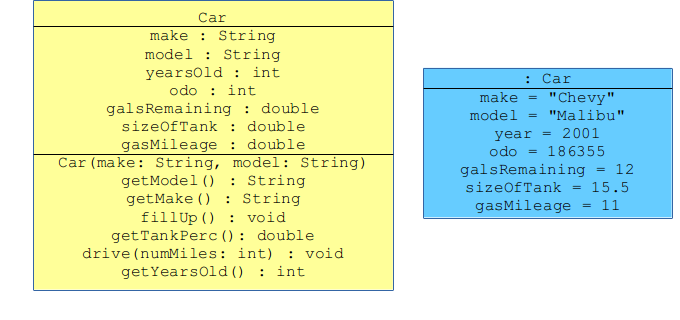
\includegraphics[width=1.0\textwidth]{classObject.pdf}   % 650x350
\caption{A class (left) and an object in UML.}
\label{fig:classObject}
\end{figure}

\subsection{Classes in UML: the first two compartments}

\index{capitalization}
Let's look at the class in detail. In the top box is its name; so far so good.
One thing to point out, though, is that in Java, \textit{the names of all
classes are \underline{capitalized}.} Don't ever violate this rule, for
convention's and confusion's sake!

\index{instance variables (inst vars)}
The second compartment has the class's \textbf{instance variables}. You'll
hear people use other terms for these like like ``member variables'' and even
``class variables,'' but I strongly prefer instance variables (or ``inst
vars'' for short) and here's why: \textit{every instance of a class has its
own copy of its instance variables.} This truth is absolutely fundamental to
OOP, and it's worth re-reading that sentence again and again until it's part
of your core being. Declaring a plain-ol' variable like ``\texttt{int x;}''
creates a single storage location in which a value can be stored. But
declaring an \textit{instance} variable is a far-reaching choice that destines
every \texttt{Car} (or whatever) that will come about in the future to have
its own copy of that variable. It's our way of defining the very structure of
Cars in perpetuity.

One slight headache is that the UML syntax differs from Java's a bit: instead
of listing the variable's type and then its name, we reverse them, we use
a colon instead of a space, and we omit the semicolon. Otherwise, it's pretty
straightforward to interpret that second compartment.

\index{class variable}
\index{underlined}
\index{car@\texttt{Car}}
\index{static@\texttt{static}}
By the way, one important piece of syntax in that second compartment is an
\underline{underline}. If an inst var is underlined, then it actually isn't an
``instance variable'' after all: it's a \textbf{class variable}. This means
that \textit{there's only one shared variable for the entire class, rather
than a different variable for each object.} In Figure~\ref{fig:classObject},
the integer \texttt{num} variable is the only underlined one. So even though
every \texttt{Car} has its own \texttt{make}, \texttt{model},
\texttt{odo}meter reading, \textit{etc.}, they all share one \texttt{num}
(which presumably represents the total number of \texttt{Car} objects
instantiated so far.) This makes sense, since after all such a variable is not
specific to a certain \texttt{Car}. We'll see that in Java, class variables
are created by using the ``\texttt{static}'' keyword where the variable is
declared.

\subsection{Classes in UML: the third compartment}

\index{method}
\index{member function}
The third compartment isn't much harder: it contains the \textbf{methods} for
the class. Like everything it seems, programmers have multiple terms for these
two: they're called \textbf{member functions} or \textbf{class functions} on
occasion. We'll stick with \textbf{method}.

\subsubsection{Functions vs. methods}

\index{function}
The crucial distinction between a method and a regular ol' Joe function is
this: while you can simply call a function to trigger it, you must call a
method \textit{on an object}. In the example, we have a \texttt{fillUp()}
method defined on the \texttt{Car} class. Since it's not an ordinary function,
but rather an OO method, we must call it on a particular instance of a
\texttt{Car}. In Java code, this does \textit{not} work:

\begin{verbatim}
    fillUp();        // NOPE
\end{verbatim}

nor does this:

\begin{verbatim}
    Car.fillUp();    // NOPE
\end{verbatim}

Instead, one must call \texttt{fillUp()} like this:

\begin{verbatim}
    johnsMercedes.fillUp();     // Correct!
\end{verbatim}

where \texttt{johnsMercedes} is the name of a valid \texttt{Car} object,
previously instantiated.

Beginners sometimes view this as a syntactic nuisance. It is not. It is
fundamental to what your code \textit{means}. Conceptually, it makes sense to
have a particular car, and to fill it up. It does \textit{not} make sense to
say ``hey universe, fill up cars'' (which is what ``\texttt{fillUp()}'' seems to
say) nor to say ``hey Cars-in-general, fill yourself up'' (which is what
``\texttt{Car.fillUp()}'' seems to say).

\index{capitalized}
By the way, notice in the example I just gave, \texttt{johnsMercedes} is
\textit{not} capitalized. (The capital ``\texttt{M}'' in the middle doesn't
count; that's just an artifact of CamelCase, which is a way of making multiple
words easier to read.) This is \textit{always} true: in Java, object names
should always begin with a lower-case letter.

Back to the third compartment. You can probably tell that the stuff inside the
parentheses is arguments to the respective methods, with the same
name-first-then-type colon-syntax, and you can probably tell that after the
closing parenthesis, you have the return type of the function. All of this
looks vaguely Java-like, and that's because even though a UML diagram is
technically programming-language-independent, language-specific things like
\texttt{int} and \texttt{String} can't help but creep in in practice. Our
thoughts betray us.

\subsubsection{Various ``special'' methods}
\label{page:instantiateConstructor}

\index{constructor}
\index{void@\texttt{void}}
A few of those methods are worthy of special note. The first one listed,
called simply ``\texttt{Car}'', is a very special kind of method called a
\textbf{constructor} which we'll be talking about a lot. Here's an iron-clad
rule which is fundamental to much that follows: \textit{whenever an object is
instantiated, one of its class's constructors is called.} This happens
automatically; it's not something we have to do ourselves. (Java's syntax for
this, as we'll see, makes it kind of look like we're calling the constructor
ourselves, which is a mixed blessing.) In Java, there are two things that
``make'' a method a constructor: (1) it must have exactly the same name as the
class, and (2) it must have \textit{no} return type. (Note that ``no'' return
type is not the same as a \texttt{void} return type! I mean \textit{no return
type at all.}\footnote{If you mistakenly include a \texttt{void} before your
constructor when you write the code, it is officially no longer a constructor!
It's now just an ordinary method -- weirdly named the same as the name of the
class it's in -- which will not be automatically invoked at instantiation time
as a constructor should. I once had a nasty bug at the eleventh hour of a
software release because of this exact issue.})

By the way, just as a class can have multiple methods with the same name as
long as those methods have different argument lists, so it can have multiple
constructors subject to the same conditions. This is a very common practice,
although in this first example we have only one \texttt{Car} constructor.

\index{underlined}
\index{numCars@\texttt{numCars()}}
Also, just as in the second compartment, an \underline{underline} indicates
that the method ``goes with the whole class, not with each object.'' And just
as before, this implies the use of the \texttt{static} keyword. A
\texttt{static} method is essentially a function: \textit{i.e.}, you
\textit{don't} call it on an object. Instead, you just call it \textit{on the
class itself.} In the example above, \texttt{numCars()} method is
\texttt{static}, which means that you could write ``\texttt{Cars.numCars()}''
to retrieve the number of \texttt{Car} objects that have been instantiated to
that point. Static methods are quite rare, but they do arise occasionally, and
are always indicated with an underline.

\index{getter}
\index{setter}
\index{mutator}
\index{accessor}
The other methods I'll draw your attention to are the ones that begin with
``\texttt{get}''. People call these methods ``\textbf{getters},'' and all they
normally do is return the value of the instance variable in question. Often
one also has ``\texttt{set}'' methods to set the values of inst vars, although
our example doesn't have any of those. Btw, some people also call getters and
setters \textbf{accessors}, and sometimes specifically call setters
``\textbf{mutators},'' a term which always made me chuckle.

\subsection{Objects in UML}

\index{object}
\index{state}
Now let's examine the blue box in Figure~\ref{fig:classObject}, which
represents an object rather than a class. It has only two compartments, not
three. That's because there's no need (in most OO languages) to say anything
about an object's methods when focusing on the object: after all, the methods
are simply defined by the class, and are common to all instances of that
class. It is important, however, to specify the current \textbf{state} of the
object, which means the current values of all its instance variables. In the
picture, you can see that there is a \texttt{Car} object in memory
representing an old Chevy Malibu with a zillion miles on it and other
suboptimal features.

\index{names}
Perhaps the strangest thing about a UML object is the top compartment. Notice
that it says ``\texttt{:~Car}'' (``colon-Car''), which is not a typo. Here's
the sitch. The top compartment of a \textit{class} has the class's name, since
that's all there is to say about it. The top compartment of an \textit{object},
meanwhile, has the \textit{object's} name, followed by a colon and then its
class. Just like we said ``\texttt{make :~String}'' earlier, so here we can
say ``\texttt{johnsMercedes :~Car}''. Why, then, is
Figure~\ref{fig:classObject} missing the name before the colon? Because we've
chosen \textit{not to name this object in the diagram.} It's just ``a Car''
with certain properties, not a named Car. This may seem odd, but in fact 99\%
of the time we will do exactly this. And that's because bizarrely,
\textit{objects don't have names in Java}, even though it may seem at first
that they do.

More on that later. For now, just accept the fact that UML diagrams can depict
objects, and normally we don't choose to specify the object's name -- only its
type and its instance variable values.


\subsection{The value of ``design''}

\index{design}
\index{class diagram}
\index{blueprint}
Before we move on to implementation, take a step back for a moment and
consider the \textit{information} contained in that
Figure~\ref{fig:classObject}.

Suppose you were given the job to write a car maintenance tracking program,
and you were getting started figuring out how to accomplish that. I think
you'll agree that if someone handed you that diagram, it would be valuable
indeed. There's no code in it \textit{per se}, but a great deal of the work
has already been done for you! You already know what to name your class, the
names and types of all its constituent variables, and what methods its objects
should support. With that diagram alone, I'd say 70\% of the work has been
done. All it takes now is to convert that diagram into Java (or whatever
language you're working with), and flesh out the methods to do the right
thing. But the overall blueprint communicates a ton of information about
decisions that have already been made. Your structure is defined, and now you
just need to bust out a hammer and some nails.


\section{Classes in Java}

\index{class@\texttt{class}}
\index{java file@\texttt{.java} file}
\index{vim@\texttt{vim}}
In Java, every class is in its own file\footnote{Technically there can be
some exceptions to this, but don't worry about them now.} named the same as
the name of the class (including the capital letter) with a \texttt{.java}
extension. Operationally, we can use \texttt{vim} to create it and edit it:

\begin{verbatim}
$ vim  Car.java
\end{verbatim}

\index{package@\texttt{package} statement}
\index{import@\texttt{import} statement}
% TODO: *Do* we actually talk about "package statements" later?
The skeleton of any class file -- after the \texttt{package} and
\texttt{import} statements we'll talk about later -- is the class definition,
with curly braces:

\begin{Verbatim}[samepage=true,fontsize=\footnotesize,frame=single]
class Car {
    
}
\end{Verbatim}

\index{public@\texttt{public}}
You may be used to putting the word ``\texttt{public}'' before the word
\texttt{class} here. For now, we won't do this, and I'll encourage you to
ditch the habit of making classes \texttt{public} by knee-jerk reaction. As
we'll learn, you want to lean towards making things ``as private as possible''
until you have reason to do otherwise.

\subsection{Instance variables in Java}

\index{instance variables (inst vars)}
Instance variables go directly inside the class definition, and outside of any
method:

\begin{Verbatim}[samepage=true,fontsize=\footnotesize,frame=single]
class Car {
    String make, model;
    int yearsOld;
    int odo;
    double galsRemaining;
    double sizeOfTank;
    double gasMileage;    
}
\end{Verbatim}

\index{private@\texttt{private}}
You may be used to seeing the word ``\texttt{private}'' before each instance
variable, and I do applaud that practice. More on that later. For now, we'll
leave it off just because it's not necessary to compile. Realize that it's not
the word \texttt{private} that makes something an instance variable; rather,
it's the fact that it's defined directly inside the class, rather than within
a method.

\subsection{Constructors in Java}

\index{constructor}
Next on the diagram is our constructor. We put in the boilerplate to get us
started:

\begin{Verbatim}[samepage=true,fontsize=\footnotesize,frame=single]
class Car {
    ...

    Car(String make, String model) {

    }
}
\end{Verbatim}

and now for the first time we have to actually think.

A constructor, as I said, is automatically called whenever an object comes
into existence. This is our ``hook'' to set up the object for success when
methods are called on it later. Think of it this way: your constructor is
called whenever a new object is about to come off the assembly line and enter
the real world. Your job in the constructor is to do everything necessary to
make sure it's ready for prime time.

Often this will involve initializing the instance variables to reasonable
values. Sometimes it will include other things, like registering its existence
in some global repository of objects, or initializing a connection to a
network, or writing itself to a database. The key question to ask yourself is,
``what do I need to do to ensure this object is `legit' and doesn't break
anything when it's being used?''

\subsection{Analyze \texttt{this}}

\index{this@\texttt{this}}
In our case, initializing the instance variables are all we need to do in the
constructor. First, let's set the object's \texttt{make} and \texttt{model} to
what was passed:

\begin{Verbatim}[samepage=true,fontsize=\footnotesize,frame=single]
class Car {
    ...

    Car(String make, String model) {
        this.make = make;
        this.model = model;
    }
}
\end{Verbatim}
\normalsize

\index{Gosling, James}
If this is the first time you've seen the odd word ``\texttt{this}'' in a
program, have a good chuckle. What a weird word choice! But Gosling \&
Co.~chose this word to denote a central OO programming concept. The word
``\texttt{this}'' means one of two different things, and they both need to be
memorized:

\begin{enumerate}
\large
\itemsep.1em
\item Inside a \textit{constructor}, ``\texttt{this}'' means ``the object that is
currently being instantiated.''
\item Inside a \textit{method}, ``\texttt{this}'' means ``the object the
method was called on.''
\item[-.] (Anywhere else, ``\texttt{this}'' is illegal.)
\normalsize
\end{enumerate}

It's weird and meta and self-referential, but it's also necessary. There are
times when we need to have a name for ``the very object I'm `in' right now,''
and ``\texttt{this}'' is our (awkward) name to refer to that.

So in our constructor, when we say ``\texttt{this.make}'' we mean ``the
\texttt{make} instance variable of this very object that is in the process of
being birthed.'' We set that to the \texttt{make} argument that was passed to
the constructor. Ditto with \texttt{model}. Oftentimes, using \texttt{this} is
optional, but in the present case it's required because we named our argument
the same as the instance variable, and there has to be a way to distinguish
between the two.

\index{initialization}
Now for our other inst vars. Some of them make sense to be set to zero:

\begin{Verbatim}[samepage=true,fontsize=\footnotesize,frame=single]
class Car {
    ...
    Car(String make, String model) {
        this.make = make;
        this.model = model;
        this.yearsOld = 0;
        this.odo = 0;
        this.galsRemaining = 0.0;
    }
}
\end{Verbatim}

since brand new cars are in fact zero years old, have a 000000 odometer, and
have no gas in their tank (maybe). Zero values for the other two don't make
sense, however; brand new cars still have a gas tank of a certain size, and
they certainly get more than 0 mpg. For this example, I'm going to go with a
very limited notion of automotive properties:

\begin{Verbatim}[samepage=true,fontsize=\footnotesize,frame=single]
class Car {
    ...
    Car(String make, String model) {
        this.make = make;
        this.model = model;
        this.yearsOld = 0;
        this.odo = 0;
        this.galsRemaining = 0.0;
        
        if (make.equals("Chevy") || make.equals("GM")) {
            sizeOfTank = 21;
        } else {
            sizeOfTank = 13;
        }
        if (make.equals("Chevy") && model.equals("Malibu")) {
            gasMileage = 3;
        } else {
            gasMileage = 24;
        }
    }
}
\end{Verbatim}

I'm totally not bitter about my car's gas mileage, by the way.

\subsection{Methods in Java}

The other methods follow a similar syntactic pattern. But it's super important
to keep this truth in the front of your mind: \textit{because they are methods
(not functions), they are called \underline{on an object.}} That means that
you can refer to instance variables inside of them -- and when you do, you're
talking about \textit{the instance variables of the object the method was
called on.} Put another way, you're talking about the instance variables of
\texttt{this}.

\subsubsection{``Client code'' and thinking reactively}

When you write methods in an OO program, you have to think reactively, not
proactively. What I mean is this. When you write a procedural, old school
program, you're the one in control. You set the agenda. In your
\texttt{main()} you say, ``first do this, then do that; create these three
variables, perform a computation, and then print the result.''

We all learned how to program this way. But in OO, you kind of have to think
backwards from that. Writing a method isn't like calling it; instead of giving
orders, you're providing a service to whoever called you. So when you write a
method, you have to think, ``okay, some other part of the code is now calling
me, for reasons of its own. What do I do in response to that?''

\index{client code}
Our term for ``that other part of the code that is now calling me'' is
\textbf{client code} (or sometimes just ``a \textbf{client}.'') The word
``client'' is used in a lot of different ways in high-tech, but here we just
mean ``the code that wants to use a particular object.'' The word connotes a
respected customer, whom we want to treat well. Very well, some client code
calls one of our methods. How should we react?

\index{state}
Often we'll react by updating the object's \textbf{state} to reflect what
should happen to it as a result of the method being called. Sometimes we'll
produce (return) a value that is stored by the object in question or
computed on the fly. Other times we'll trigger some side effect, like printing
to the screen, writing to a database, or calling some \textit{other} method(s)
on the same or a different object.

\index{implement}
\index{fillUp@\texttt{.fillUp()}}
This is best seen through examples. Let's implement\footnote{The verb
\textbf{to implement} means ``to take a design and actually build it out.'' It
is a synonym for the verb \textbf{to code}.} the \texttt{.fillUp()} method
first. Don't think about Java; think about cars. If I fill up a car, what
happens?

Does the make or model or mileage change? Of course not: the amount of gas in
the tank does. And ``fill 'er up'' means to raise it to its maximum. The
correct implementation of \texttt{.fillUp()}, then, is simply:

\begin{Verbatim}[samepage=true,fontsize=\scriptsize,frame=single]
class Car {
    ...
    void fillUp() {
        galsRemaining = sizeOfTank;
    }
}
\end{Verbatim}

We could equally well have written this as:

\begin{Verbatim}[samepage=true,fontsize=\scriptsize,frame=single]
class Car {
    ...
    void fillUp() {
        this.galsRemaining = this.sizeOfTank;
    }
}
\end{Verbatim}

to make it explicit that we're talking about two instance variables here, and
assigning the value of one to the other. It's a matter of style.

In the same vein, we ask ourselves, ``suppose some client code asks me what
percentage full my tank is. What answer do I give them?'' The proper response
involves these same two inst vars and a little math:

\begin{Verbatim}[samepage=true,fontsize=\scriptsize,frame=single]
class Car {
    ...
    double getTankPerc() {
        return galsRemaining / sizeOfTank * 100;
    }
}
\end{Verbatim}

I chose to omit \texttt{this}, but again it's a personal choice.

Some methods are no-brainers:

\begin{Verbatim}[samepage=true,fontsize=\scriptsize,frame=single]
class Car {
    ...
    String getModel() {
        return model;
    }
}
\end{Verbatim}

If a client asks me what my model is, I tell them my model, duh. The same is
true for the other accessor methods.

\index{drive@\texttt{.drive()}}
Finally, what if a client instructs me to drive $n$ miles? How should my
internal state be adjusted to reflect that?

This is the most difficult one, and again it requires you to think about cars
rather than about Java. Mentally run through the variables we've chosen to
represent a car, and ask yourself which ones need to change, and how? You'll
realize that the odometer and the gas tank level are the two we need to
modify. When someone drives a car $n$ miles, the odometer needs to increase by
$n$ miles (else it ain't legal); also, the gas tank needs to be reduced by
$\frac{n}{m}$ gallons, where $m$ is the car's gas mileage in mpg. So here we
go:

\begin{Verbatim}[samepage=true,fontsize=\footnotesize,frame=single]
class Car {
    ...
    void drive(int numMiles) {
        double galsBurned = numMiles / this.gasMileage;
        this.galsRemaining = this.galsRemaining - galsBurned;
        this.odo += numMiles;
    }
}
\end{Verbatim}

This time, I did include the \texttt{this}'s where appropriate, since we also
have a couple of local variables involved and I wanted to be explicit. Our
math is a mix of function parameters, temporary variables, and permanent
attributes of the \texttt{Car}.


\section{Objects in Java}

\index{object}
We've now coded a class from the ground up (the complete code listing is in
Figure~\ref{fig:carClassCodePreExceptions}.) We did this so clients can
instantiate objects of that type and do something with them. Let's make a
simple \texttt{main()} method to do just that.

You'd be surprised how many beginning programmers try to drive 23 miles like
this:

\begin{Verbatim}[samepage=true,fontsize=\scriptsize,frame=single]
    public static void main(String args[]) {
        drive(23);    // WRONG!
    }
\end{Verbatim}

or this:

\begin{Verbatim}[samepage=true,fontsize=\scriptsize,frame=single]
    public static void main(String args[]) {
        Car.drive(23);    // equally WRONG!
    }
\end{Verbatim}

Yes you'll get compiler errors, but those errors reflect a deeper and more
fundamental misunderstanding. In OOP, you have to call a method \textit{on an
object}. Conceptually, nothing else makes sense. In real life you don't
``drive in general,'' and you don't ask ``automobiles in general'' to drive
you places. Instead, you have to drive \textit{a particular car} somewhere.
Here's how:

\begin{Verbatim}[samepage=true,fontsize=\scriptsize,frame=single]
    public static void main(String args[]) {
        Car minivan = new Car("Toyota","Sienna");
        minivan.drive(23);    // correct!
    }
\end{Verbatim}

\index{new@\texttt{new}}
\index{instantiate}
The keyword ``\texttt{new}'' is utterly crucial here. In Java, \textit{the only
way to instantiate an object is to use \texttt{new}}. It causes a fresh object
of the appropriate type to spring into existence, complete with memory to hold
its instance variables. And the appropriate constructor is called, of course,
to set that object up for prime time.

We got errors before because we didn't even \textit{have} a car to do anything
with. There was no memory set aside, no constructor called to set up the
object, nothing. We tried a shortcut, and that was madness. But now that we
know how to instantiate objects, we can do so to several and create a whole
new world, as in Figure~\ref{fig:wholeNewWorld} on
p.~\pageref{fig:wholeNewWorld}. All the code in that figure is legit, and
shows that our \texttt{Car} class has uses.

\begin{figure}[h]
\centering
\begin{Verbatim}[samepage=true,fontsize=\footnotesize,frame=single]
    public static void main(String args[]) {

        // The archaic Davies family vehicles
        Car minivan = new Car("Toyota","Sienna");
        minivan.setYear(2002);
        Car stephensLemon = new Car("Chevy","Malibu");
        minivan.setYear(2001);

        // Grammy lives in Colorado
        Car grammysCar = new Car("Lexus","ES");
        grammysCar.setYear(2018);

        // Caravan to Disneyworld -- whoo-hoo!  (Grammy's meeting us there.)
        minivan.fillUp();
        minivan.drive(500);
        stephensLemon.fillUp();
        stephensLemon.drive(500);
        System.out.println("The van is " + minivan.getTankPerc() + 
            "% full, while the chevy is " + stephensLemon.getTankPerc() +
            "% full.");
        grammysCar.drive(1899);  // a long way from Colorado
    }
\end{Verbatim}
\caption{A client \texttt{main()} program that uses the \texttt{Car} class.}
\label{fig:wholeNewWorld}
\end{figure}


\subsection{Printing an object}

One last thing before we bring this chapter to a close. Suppose we're
debugging our program, and we want to print out the values of various
variables to help us hunt down an error. Printing an \texttt{int} or other
standard type is straightforward:

\begin{Verbatim}[samepage=true,fontsize=\scriptsize,frame=single]
    int numEnchiladas = 3;
    System.out.println("The number of enchiladas is: " + numEnchiladas + ".");
\end{Verbatim}

and will produce a message like ``\texttt{The number of enchiladas is 3.}''
What happens, though, if we print out an \textit{object}, like a \texttt{Car}?
How can such a complex entity be reduced to a string of text?

Heck, let's try it:

\begin{Verbatim}[samepage=true,fontsize=\scriptsize,frame=single]
    Car porsche = new Car("Porsche","Carrera");
    porsche.setYearsOld(2);
    System.out.println("My car is: " + porsche + ".");
\end{Verbatim}

The output we get is:

\begin{verbatim}
   My car is: Car@4aa298b7.
\end{verbatim}

Whoa. The word ``\texttt{Car}'' is perhaps not surprising, but what's the rest
of that gunk?

\index{memory address}
It turns out that Java's default way of rendering an object as a
\texttt{String} is to concatenate the name of the class, an ``at'' sign,
followed by \textit{the memory address} in which it is stored. We'll talk much
more about memory in the next chapter. For now, just think of the memory
address as a unique number\footnote{Yes, it is indeed a number, despite the
fact that it has letters in it like '\texttt{a}' and '\texttt{b}'. It's
printed here in \textbf{hexadecimal}, which is a base-16 number system instead
of the base-10 system non-computer-science humans use.} that identifies the
object, like an SSN.

\begin{samepage}
\label{pg:toString}
\index{override}
\index{toString@\texttt{.toString()}}
The cool thing is, we can \textbf{override} this functionality at will, and
change the way \texttt{Car}s will be printed. Check it out. Create a method in
the \texttt{Car} class called \texttt{.toString()}. It must:

\begin{compactenum}
\itemsep.1em
\item be called exactly ``\texttt{.toString()}''.
\item take no argument.
\item return a \texttt{String}.
\index{public@\texttt{public}}
\item have the word \texttt{public} immediately before the return type. (We'll
talk a lot about what \texttt{public} means in future chapters. For now, it just has to
be there.)
\end{compactenum}
\end{samepage}

Here's one:

\begin{Verbatim}[samepage=true,fontsize=\scriptsize,frame=single]
    public String toString() {
        return "a " + yearsOld + "-year-old " + make + " " + model;
    }
\end{Verbatim}

We're assembling various aspects of the vehicle into a sensible, readable
string. Now, when we run \textit{the same code} as above, our output is this:

\begin{verbatim}
   My car is: a 2-year-old Porsche Carrera.
\end{verbatim}

Notice that we didn't explicitly ever call \texttt{.toString()}! Instead, we
just used a \texttt{Car} object in a context in which a \texttt{String} was
required, and Java faithfully called our method instead of the one that
generated the memory address. Pretty cool.

\texttt{inheritance}
This is actually our first foray into a really deep and powerful technique
called ``inheritance,'' about which much more will come in later chapters. For
now, just grasp the idea that Java lets us override its general behavior for
specific kinds of objects, which gives us tremendous power and flexibility.

\begin{figure}
\begin{Verbatim}[fontsize=\scriptsize,frame=single]
class Car {
    String make, model;
    int yearsOld, odo;
    double galsRemaining, sizeOfTank, gasMileage;

    Car(String make, String model) {
        this.make = make;
        this.model = model;
        yearsOld = 0;
        odo = 0;
        galsRemaining = 0;
        if (make.equals("Chevy") || make.equals("GM")) {
            sizeOfTank = 21;
        } else {
            sizeOfTank = 13;
        }
        if (make.equals("Chevy") && model.equals("Malibu")) {
            gasMileage = 3;
        } else {
            gasMileage = 24;
        }
    }

    public String toString() {
        return "a " + yearsOld + "-year-old " + make + " " + model;
    }

    String getMake() { return make; }

    String getModel() { return model; }

    int getYearsOld() { return yearsOld; }

    void setYearsOld(int x) { yearsOld = x; }

    void fillUp() {
        this.galsRemaining = this.sizeOfTank;
    }

    double getTankPerc() {
        double perc = galsRemaining / sizeOfTank * 100;
        return perc;
    }

    void drive(int numMiles) {
        double galsBurned = numMiles / gasMileage;
        galsRemaining = galsRemaining - galsBurned;
        odo += numMiles;
    }
}
\end{Verbatim}
\caption{A complete Java implementation of the \texttt{Car} class.}
\label{fig:carClassCodePreExceptions}
\end{figure}


\backmatter
\printindex

\end{document}
